\documentclass[../../main.tex]{subfiles}
 
\begin{document}

What follows is a short numerical analysis of student evaluation data from Tab. \ref{tab:courses:intro_eval_1}-\ref{tab:courses:adv_eval_2}.  The \textit{mean scores} for questions 10-15 are plotted on the x-axis of Fig. \ref{fig:ag_data} (left) for introductory courses I taught in Fall 2017, and on the x-axis of Fig. \ref{fig:ag_data} (right) for Spring 2018.  The \textit{mean} is synonymous with the average of the data.  The \textit{standard deviation} measures how much the data varies within the data set, around the mean.  We can find the \textit{fractional error} of a measured mean by dividing the standard deviation by the mean.  For example, a score with a mean of 4.0 and a standard deviation of 2.0 has a fractional error of 2.0/4.0 or 50\%. If a measurement has large fractional error, there is less consensus and more variation.  Similarly, if the data show a low fractional error, there is consensus toward the mean. \\ \hspace{0.1cm}

In general, when the scores are lower in a particular category, there are larger standard deviations.  When I score high, my students are in closer alignment with each other.  One way of showing this numerically is Fig. \ref{fig:ag_data}.  For both Fall and Spring courses, the standard deviation for the scores is inversely correlated with the mean scores.  The fractional error is typically $\approx 50$\% for low scores.  This is large when compared to the $10$\% when the scores are high.  A subset of students must have been marking low scores, while the rest were marking high scores (this the only way to obtain a such standard deviations).  A linear regression, or trend line, has been matched to the data in Fig. \ref{fig:ag_data}, and shows that that the standard deviation is inversely correlated with mean score.  This is further evidence that there is more consensus when the scores are higher, and vice versa when they are lower.

\begin{figure}[ht]
\centering
\includegraphics[width=0.33\textwidth,angle=270]{aggregate_data_fall_2017_intro.eps}
\includegraphics[width=0.33\textwidth,angle=270]{aggregate_data_spring_2018_intro.eps}
\caption{\label{fig:ag_data} (Left) Aggregate standard deviations versus mean scores for questions 10-25 for introductory courses taught in Fall 2017.  (Right) Same, for introductory courses taught in Spring 2018.}
\end{figure}

My hypothesis is that the individual students causing the large standard deviations and lower means are the ones who are struggling with the material.  \textit{By locating the struggling students and providing one-on-one discussion time with them, I hope to push the data points further into the lower right corners of Fig. \ref{fig:ag_data}}.  This would indicate more student satisfaction, and more consensus.  The students needing attention are more likely to rate the course and professor more favorably if their needs are met.  I outline three concrete steps to achieve this in Sec. \ref{sec:oof}.

\end{document}
